% !TEX TS-program = pdflatex
% !TEX encoding = UTF-8 Unicode

% This is a simple template for a LaTeX document using the "article" class.
% See "book", "report", "letter" for other types of document.

\documentclass[12pt]{article} % use larger type; default would be 10pt
\usepackage{color}
\usepackage[utf8]{inputenc} % set input encoding (not needed with XeLaTeX)

%%% Examples of Article customizations
% These packages are optional, depending whether you want the features they provide.
% See the LaTeX Companion or other references for full information.

%%% PAGE DIMENSIONS

\usepackage[top=20mm,right=20mm,bottom=15mm,left=20mm]{geometry}
% \geometry{margins=2in} % for example, change the margins to 2 inches all round
% \geometry{landscape} % set up the page for landscape
%   read geometry.pdf for detailed page layout information

\usepackage{graphicx} % support the \includegraphics command and options

% \usepackage[parfill]{parskip} % Activate to begin paragraphs with an empty line rather than an indent

%%% PACKAGES
\usepackage{booktabs} % for much better looking tables
\usepackage{array} % for better arrays (eg matrices) in maths
%\usepackage{paralist} % very flexible & customisable lists (eg. enumerate/itemize, etc.)

%\usepackage{subfig} % make it possible to include more than one captioned figure/table in a single float
\usepackage{amsfonts}
\usepackage{amsthm}
\usepackage{tikz}
\usepackage{amsmath}
\usepackage{float}
\usepackage{graphicx}
\usepackage{caption}
\usepackage{subcaption}
\usepackage{color}

% These packages are all incorporated in the memoir class to one degree or another...

%%% HEADERS & FOOTERS
\usepackage{fancyhdr} % This should be set AFTER setting up the page geometry
\pagestyle{fancy} % options: empty , plain , fancy
\renewcommand{\headrulewidth}{0pt} % customise the layout...
\lhead{}\chead{}\rhead{}
\lfoot{}\cfoot{\thepage}\rfoot{}

%%% SECTION TITLE APPEARANCE
%\usepackage{sectsty}
%\allsectionsfont{\sffamily\mdseries\upshape} % (See the fntguide.pdf for font help)
% (This matches ConTeXt defaults)

%%% ToC (table of contents) APPEARANCE
%\usepackage[nottoc,notlof,notlot]{tocbibind} % Put the bibliography in the ToC
%\usepackage[titles,subfigure]{tocloft} % Alter the style of the Table of Contents
%\renewcommand{\cftsecfont}{\rmfamily\mdseries\upshape}
%\renewcommand{\cftsecpagefont}{\rmfamily\mdseries\upshape} % No bold!


\newtheorem{theorem}{Theorem} 
\newtheorem{lemma}{Lemma}
\newtheorem{propn}{Proposition}
\newtheorem*{thmm}{Theorem}
\newtheorem{remk}{Remark} 
\newtheorem{corol}{Corollary}
\newtheorem{definition}{Definition}



\newtheorem{thm}{Theorem}[section] 
\newtheorem{prop}[thm]{Proposition} 
\newtheorem{lem}[thm]{Lemma}
\newtheorem{cor}[thm]{Corollary} 
\newtheorem{con}[thm]{Conjecture} 

\theoremstyle{definition}
\newtheorem{defn}[thm]{Definition}
\newtheorem*{rem}{Remark}
%\newtheorem*{nota}{Notation}
\newtheorem*{nota}{Notation}
\newtheorem{cla}[thm]{Claim}
\newtheorem{ex}[thm]{Example}
\newtheorem{exs}[thm]{Examples}
\newtheorem*{exer}{Exercise}
\newtheorem{case}{Case}

\definecolor{sotonblue}{rgb}{0.0,0.394,0.597}
%opening
\title{Some probabilities}
\author{David Matthews}

\begin{document}

\title{Biological Trees}
\author{David Matthews}

\section{Introduction}
%leaves???
Alzheimer's disease (AD) is a debilitating medical condition that affects one in eight people over 65 years of age \cite{Bengt}.  However, precise details of the mechanism that causes AD are largely unknown.  Here we build a graph theoretic model that demonstrates the importance of symmetry of the cerebral arterial tree to the proliferation of AD.

\subsection{Medicine}

Extracellular space in the brain contains interstitial fluid (ISF) which is produced by the blood and by-products of cell metabolism.  The extracellular spaces within the walls of cerebral blood vessels referred to as \emph{basement membranes} represent the perivascular pathways along which ISF drains out of the brain \cite{wellerperi,wellermicro,Rox}.  Figure \ref{fig:1} depicts perivascular drainage of A$\beta$ along basement membranes. 

\begin{figure}[h]

              \centering
               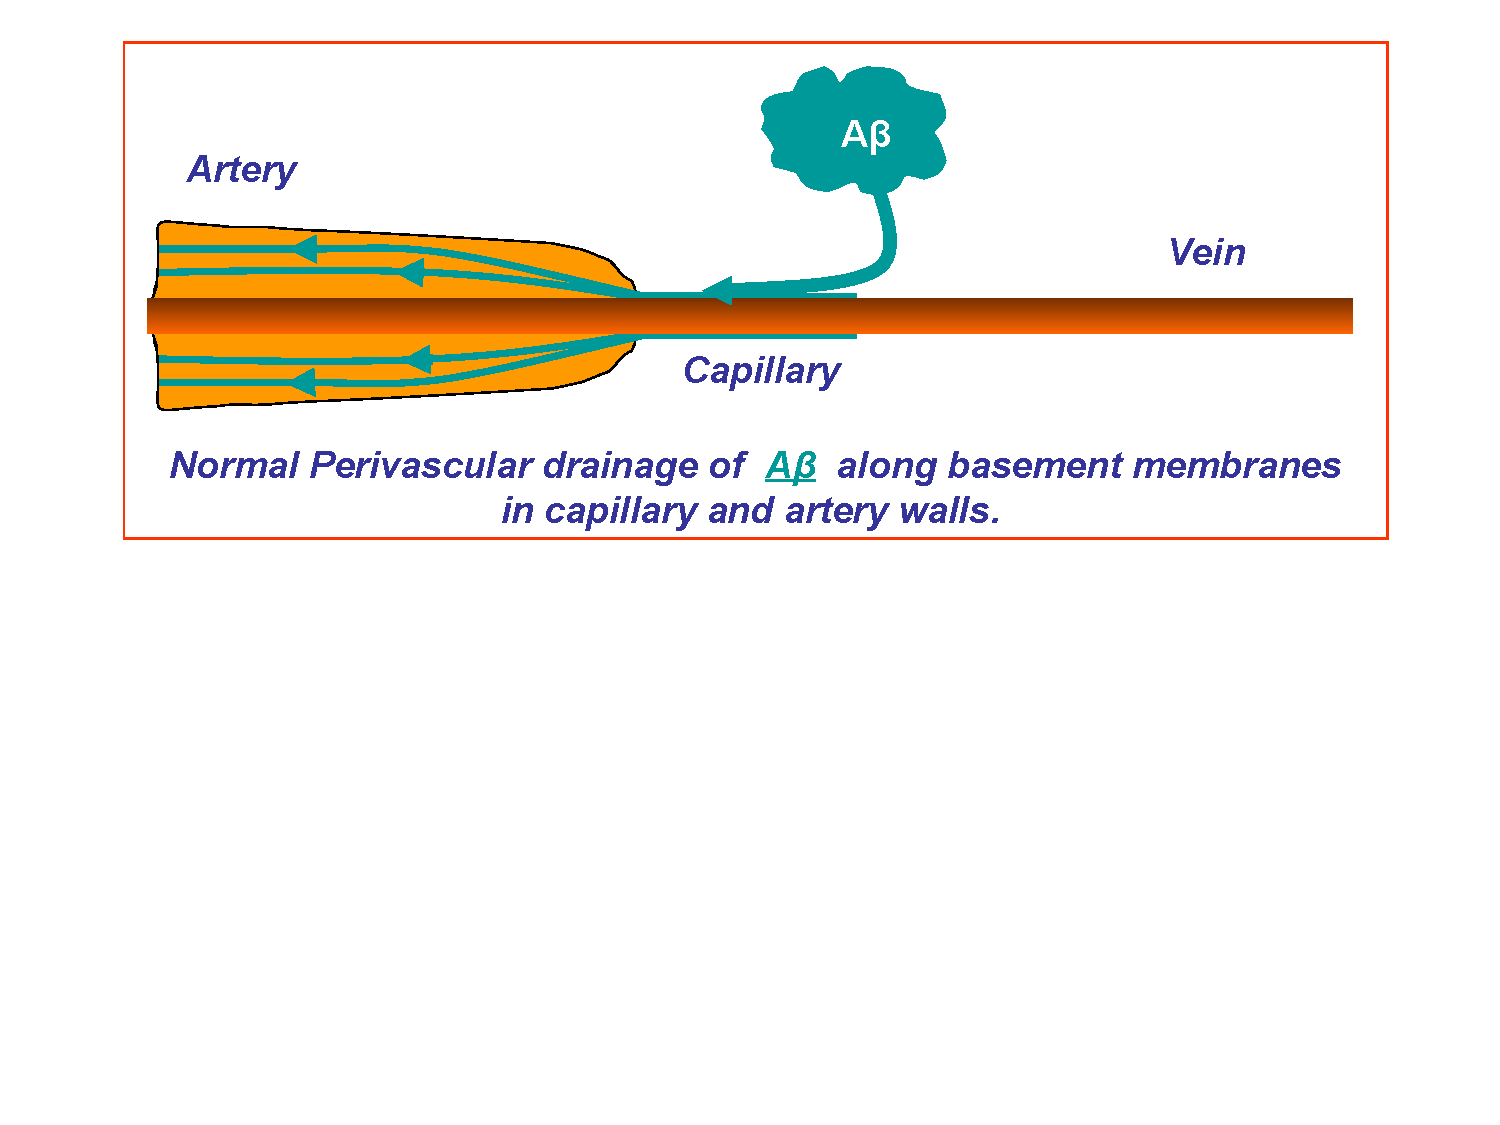
\includegraphics[scale=0.3]{PVD1.pdf}
                \caption{}\label{fig:1}
\end{figure}

The walls of cerebral capillaries consist of one fused layer of  the basement membrane which is approximately 150 nm in thickness.  

Alzheimer's disease is the most common dementia - characterised by serious and progressive cognitive decline and appears to be due to a failure of elimination of amyloid-$\beta$ (A$\beta$) from the brain.  A$\beta$ is a normal by-product of cell metabolism produced at all ages \cite{wellerperi}.

One mechanism for the removal of A$\beta$ from the brain parenchyma is perivascular drainage, by which A$\beta$ within ISF enters the capillary basement membranes draining to the walls of arteries towards the surface of the brain.  With ageing and certain genetic background soluble A$\beta$ is not eliminated from the brain and it is deposited in the walls of blood vessels as cerebral amyloid angiopathy (CAA) \cite{Rox}\cite{wellerperi}.  In Figure \ref{figy:2}  the deposition of A$\beta$ is shown in red.  

\begin{figure}

              \centering
               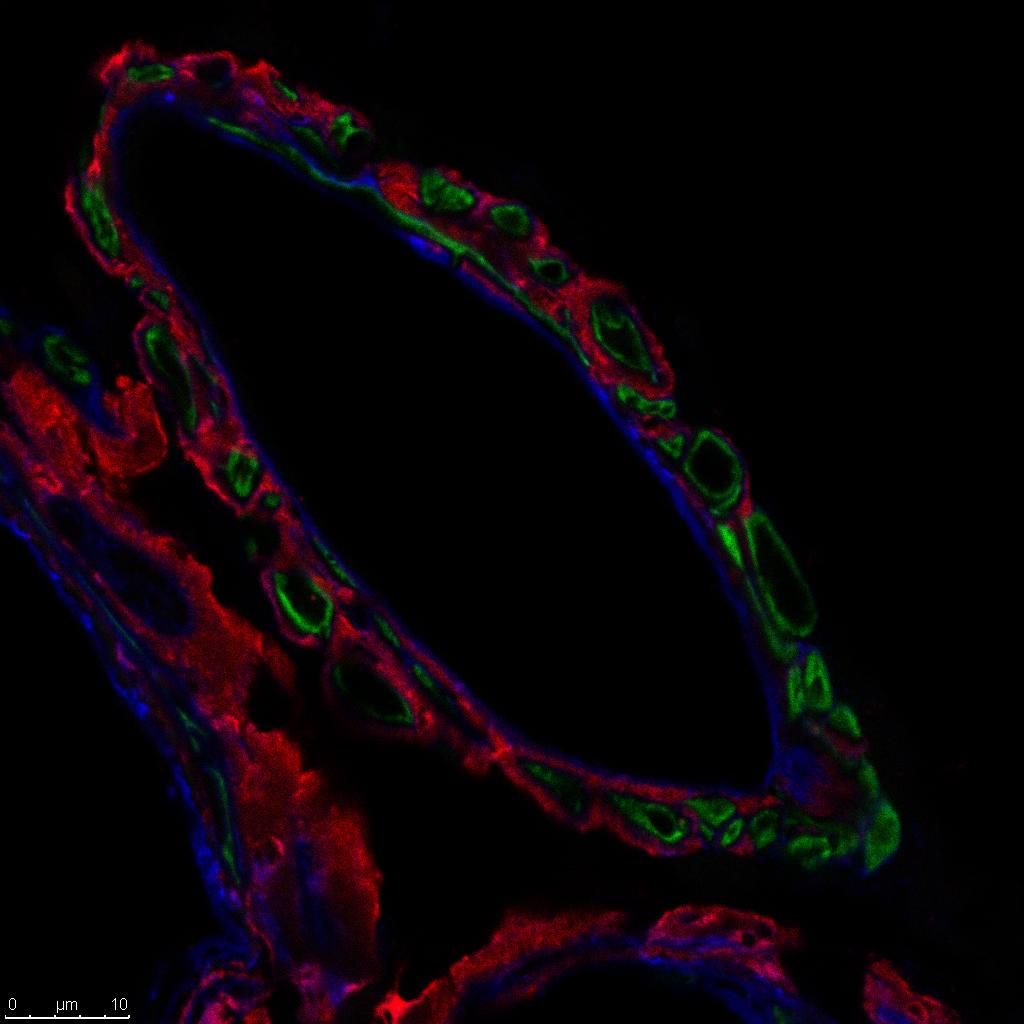
\includegraphics[scale=0.15]{abeta.jpg}
                \caption{CAA in a leptomeningeal artery.}\label{figy:2}
\end{figure}

The deposition of A$\beta$ in the perivascular spaces in the  blood vessel walls can cause a further blockage of the ISF drainage pathways resulting in an alteration of the composition of ISF in the brain parenchyma. This change in biochemical composition of the ISF leads to nerve cell death and Alzheimer's Disease. \cite{Rox}.  

CAA  is most prominent in the occipital, temporal and frontal lobes and least prominent in the parietal lobe and cerebellum.  In particular,  the leptomeningeal and cortical arteries are particularly prone to CAA whereas CAA is very rare in capillaries \cite{Preston}.  One possible reason for the differing expected degrees of CAA could be the differing topology and symmetry of the cerebral arterial tree.  In order to test this hypothesis we consider a graph theoretic model of CAA and therefore need to make some relevant definitions from graph theory.  

%link to aneurysms etc.



%precise definition of a node and a branch



\subsection{Graph Theory}\label{trees}  The references for this section are \cite{Bela} 
and \cite{varietiesofincreasintrees}.
Graph Theory has been an established area of discrete mathematics since 1736 when Euler 
solved the famous question regarding the bridges of K\"{o}nigsberg.  More recently, in the 
1940s and 50s Erd\H{o}s and R\'{e}nyi laid the foundations of the theory of random graphs 
seeking to answer fundamental questions about the nature of ``most'' graphs. Random graphs 
have been studied for their own sake and have been used to model a diverse set of real-world 
networks from the world wide web to the metabolism of \emph{E. coli} \cite{barabasi}. Recently the advent of the world wide web and the accompanying %symbiotic?
cheap and powerful computational power has led to a re-emergence of  
random graph theory under the guise of ``Network Science''. 
%Steal from your summer project especially references.
%exactly which type of trees do we mean? - see one of the papers on your desk.  

An simple undirected graph, $G$, is a pair $G = (V(G),E(G))$ where $V(G)$ is the a set of vertices or nodes of the graph and $E(G)$ is 
%a subset of unordered pairs $V(G) \times V(G)$ we call $E(G)$ 
the set of edges of $G$.  Each edge $e \in E(G)$ has two endpoints $u,v \in V(G)$ and we say that if $e = e_{u,v}$ then $u$ and $v$ are \emph{adjacent} and that $endpoints(e) = \{u,v\}$.  We do not allow more than one edge between a pair of vertices or loops which are edges $e$ such that $endpoints(e) = \{u\}$. The degree of any vertex $v$ is the number of edges $e$ such that $v \in endpoints(e)$. 
%example graph.

A tree, $T$, is a graph such that the shortest path between any pair of vertices $u,v \in V(T)$ is unique.  For example the graph in Figure \ref{fig:3} is a tree. 
\begin{figure}
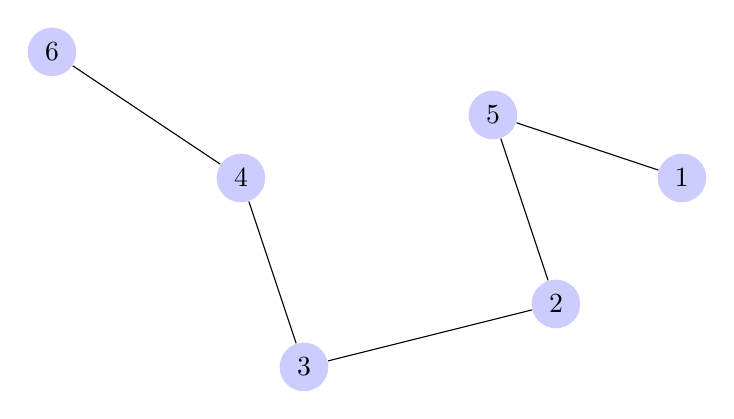
\begin{tikzpicture}
  [scale=.8,auto=left,every node/.style={circle,fill=blue!20}]
  \node (n6) at (1,10) {6};
  \node (n4) at (4,8)  {4};
  \node (n5) at (8,9)  {5};
  \node (n1) at (11,8) {1};
  \node (n2) at (9,6)  {2};
  \node (n3) at (5,5)  {3};

  \foreach \from/\to in {n6/n4,n5/n1,n2/n5,n2/n3,n3/n4}
    \draw (\from) -- (\to);

\end{tikzpicture}
 \caption{}\label{fig:3}
\end{figure}

A \emph{random recursive tree} (RRT), $T$, with vertices $V(T) = \{v_{1},\dots,v_{n}\}$ is a 
labelled, rooted tree obtained by assigning a root vertex $v_{1}$ then adding $n-1$ vertices 
one by one such that each new vertex is joined by an edge to a randomly and uniformly chosen 
existing vertex. A random recursive $q$-ary tree is a labelled, rooted tree built in the same 
way as a random recursive tree except each new vertex is attached uniformly at random to an 
existing vertex that has outdegree less than $q$ \cite{varietiesofincreasintrees}.  We say that RRTs and random 
recursive $q$-ary trees are \emph{increasing} trees.  

Given an increasing tree $T_{n}$ on $n$ vertices labelled by the function 
$\phi : V(T) \rightarrow \{1,2,\dots,n\}$ and a vertex $v \in V(T)$ then we can consider 
$\tilde{T_{v}}$  which is the induced subtree with vertices, $v_{i}\in B(v)$ such that 
$\phi(v_{i}) \geq \phi(v)$. 

Given some tree $T$ we can formally measure how \emph{symmetric} that tree is by calculating 
the number of permutations of the vertices of that graph which preserves adjacent vertices.  
We call the set of all these permutations, $Aut(T)$, the \emph{automorphism group} of $T$ and 
the number of allowed permutations, $|Aut(T)|$ is the size of the automorphism group.  

\begin{ex}
Consider the following increasing tree $T_{14}$ with 14 vertices.  
\begin{figure}[H]
\centering
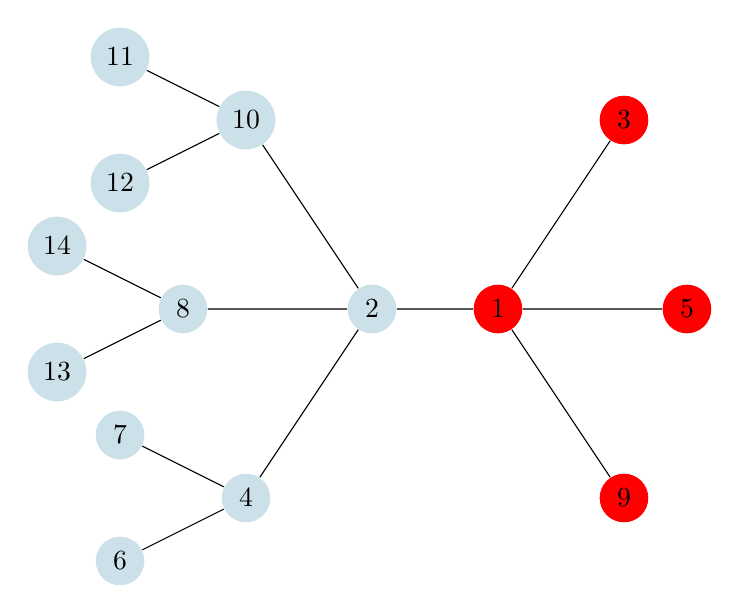
\begin{tikzpicture}
  [scale=0.8,auto=left,every node/.style={circle,fill=sotonblue!20}]

  \node[style={circle,fill=red!100}] (n1) at (7,5) {1};
  \node (n2) at (5,5)  {2};
  \node[style={circle,fill=red!100}] (n3) at (9,8)  {3};
  \node (n4) at (3,2) {4};
  \node[style={circle,fill=red!100}] (n5) at (10,5)  {5};
  \node (n6) at (1,1)  {6};
  \node (n7) at (1,3)  {7};
  \node (n8) at (2,5)  {8};
  \node[style={circle,fill=red!100}] (n9) at (9,2)  {9};considering
  \node (n10) at (3,8)  {10};
  \node (n11) at (1,9)  {11};
  \node (n12) at (1,7)  {12};
  \node (n13) at (0,4)  {13};
  \node (n14) at (0,6)  {14};
  \foreach \from/\to in {n1/n2,n1/n3,n1/n5,n1/n9,n2/n4,n2/n8,n2/n10,n10/n11,n10/n12,n8/n14,n8/n13,n4/n7,n4/n6}
    \draw (\from) -- (\to);
\end{tikzpicture}
\caption{}\label{fig2}
\end{figure}
The red vertices in Figure \ref{fig2} indicate an induced subtree $\tilde{T}_{v_{1}}$.  We can permute the 
vertices $v_{3},v_{5}$ and $v_{9}$, for example the following is a valid permutation of these 
vertices.
\begin{align*}
 3 \rightarrow 5\\
 5 \rightarrow 3\\
 9 \rightarrow 9 
\end{align*}
Note that after the above permutation all three vertices remain adjacent to $v_{1}$.  There are $3! = 6$
 distinct such permutations. The blue vertices in Figure \ref{fig2} highlight an extended 
symmetric induced subtree, 
$\tilde{T}_{v_{2}}$.  We can permute any of the pairs $\{v_{6},v_{7}\}, \{v_{11},v_{12}\}$ 
and $\{v_{13},v_{14}\}$ and we can permute the longer branches.  For example the following 
is a valid (adjacency preserving) permutation:
\begin{align*}
 4\rightarrow 8 \\
6 \rightarrow 13\\
7 \longrightarrow 14\\
8 \rightarrow 4\\
13 \rightarrow 7\\
14 \rightarrow 6
\end{align*}
Where every other vertex is fixed.  There are $X$ possible valid permutations of the blue 
vertices, therefore $|Aut(T_{14})| = 6 \times X = 6X$
\end{ex}

%ADD EXAMPLE
%\begin{tikzpicture}
%  [scale=.8,auto=left,every node/.style={circle,fill=blue!20}]
%  \node (n1) at (6,10) {1};
%  \node (n2) at (6,6)  {2};
%  \node (n3) at (2,2)  {3};
%  \node (n4) at (10,2) {4};
  

  %\foreach \from/\to in {n1/n2,n2/n3,n2/n4}
%    \draw (\from) -- (\to);

%\end{tikzpicture}

%\begin{figure}[H]
%
%              \centering
%              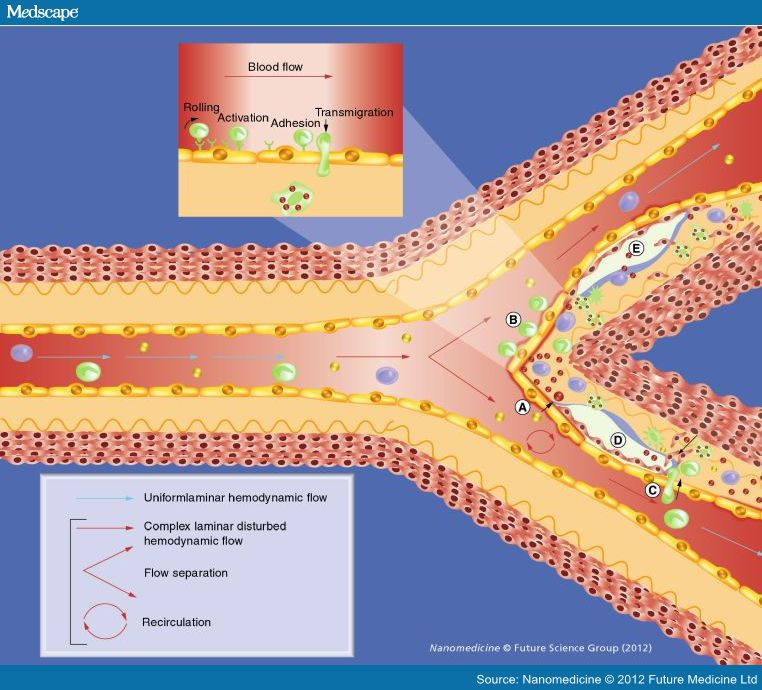
\includegraphics[scale=0.3]{bifir.jpg}
%                \caption{Perivascular drainage of A$\beta$.}
%\end{figure}
\subsubsection{Anatomical Data}\label{sec:ana}


 
In order to build an effective model we require anatomical data such as the expected length
 and radii of arterial vessels and the expected number of branching points.     

Note that 98\% of branching in the cerebral cortex is bifurcation and we expect approximately 
300 branching points \cite{Cassot}. 

Murray's principle of minimization of operational cost states that the cost of operation of
 physiological systems tends to a minimum.  One consequence of Murray’s principle is referred 
to as Murray's law which states that for $2$ daughter branches $d_{1}$ and $d_{2}$ from a 
common parent arterial vessel, $p$: 
\[r_{p}^{3} = r_{d_{1}}^{3} + r_{d_{2}}^{3}\]
where $r_{p}$ is the radius of $p$ and $r_{d_{1}},r_{d_{2}}$ are the radii of $d_{1}$ and 
$d_{2}$ \cite{Murray}.
Experimental evidence has shown that Murray's law is a good approximation for 
arterial vessels \cite{Cohn,Zamir}.

Murray's law describes the relationship between particular vessels which can be thought of as 
\emph{cylinders}.  However, recall that our goal is to model the cerebral perivascular pathways
which can be thought of as \emph{annular prisms}.  Therefore we will adjust Murray's law to describe 
the relationship between parent and child annular prisms.  Since the notion of radius is more 
complicated for an annular prism it is necessary to reformulate Murray's law in terms of 
cross-sectional area.   

We assume that the width of the perivascular space, $\epsilon$ is the same for any vessel from capillary to
 artery.  So let he parent vessel have radius $r_{p} = r_{p}' + \epsilon$ and the two 
daughter vessels have radii $r_{di} = r_{di}' + \epsilon$.
%insert diagram here
The relationship between the cross-sectional area, $A_{X}$ of any vessel and the radius, $r_{X}$ 
of that vessel is given by the formulae:
\begin{align*}
 A_{X} &= \pi((r_{X}' + \epsilon)^{2} - r_{X}'^{2})\\
 &= \pi(\epsilon^{2} + 2\epsilon r_{X}')\\
 r_{X}' &= \frac{A_{X} - \pi\epsilon^{2}}{2\epsilon\pi}\\
 r_{X} &=  \frac{A_{X} - \pi\epsilon^{2}}{2\epsilon\pi} + \epsilon \\
 &= \frac{A_{X} + \pi\epsilon^{2}}{2\epsilon\pi}
\end{align*}

By combining the above equations we find that the cross-sectional area of the parent
 vessel, $A_{p}$, is given by:

\begin{align*}
A_{p} &= \pi(\epsilon^{2} + 2\epsilon r_{p}) \\
&= \pi\left(\epsilon^{2} + 2\epsilon (r_{d_{1}}^{3} + r_{d_{2}}^{3})^{\frac{1}{3}}\right)\\
&= \pi\left(\epsilon^{2} + 2\epsilon \left(\left( \frac{A_{d_{1}} + \pi\epsilon^{2}}{2\epsilon\pi} \right)^{3} + \left( \frac{A_{d_{2}} + \pi\epsilon^{2}}{2\epsilon\pi} \right)^{3}\right)^{\frac{1}{3}}\right)
\end{align*}
%\[A_{p} = \frac{((A_{1} - \epsilon^{2})^{3} +(A_{2} - \epsilon^{2})^{3})^{\frac{1}{3}}}{\epsilon} + \pi\epsilon^{2}\]
where $A_{d_{1}}$ and $A_{d_{2}}$ are the cross-sectional areas of the two daughter vessels.
%later we will chose epsilon to be one an initially set all leaves to have radius 300



\section{Method}\label{sec:meth}

In this section we will describe the program we built using the numerical modelling program \emph{matlab} \cite{matlab} which replicates CAA.  This program has four constituent parts:
\begin{itemize}
\item[(i)]Generate a random recursive $q$-ary tree, $T^{q}_{n}$ on $n$ nodes.
\item[(ii)]Calculate $|Aut(T^{q}_{n})|$.
\item[(iii)]Dynamically remove edges of $T^{q}_{n}$ according to a predetermined probability model.
\item[(iv)]Record the time, $\tau_{\frac{1}{2}}$, to remove half of the edges from $T^{q}_{n}$ which we think of as the "half-life" of the process.
\end{itemize} 
This program was then run 50 times and we investigated the relationship between $|Aut(T_{q}^{2})|$ and $\tau_{\frac{1}{2}}$.   

In accordance with the anatomical survey paper by Cassot \emph{et al.} discussed in Section \ref{sec:ana} we set $n = 300$ and  $q=2$.  
We used the graph isomorphism program \emph{nauty} \cite{nauty} to calculate the size of the automorphism group of each tree.  

The dynamic process of edge removal can be defined as follows.  At time $t=0$ we set $T(0) = T^{2}_{300}$ our randomly generated binary tree.  At time  $t = 1,2,\dots$ for every edge  $e \in E(T(t-1))$ there is some probability $0<P\leq 1$ that $e $ is removed.  If edge $e = e_{uv}$ is removed then we also remove the induced subtree $\tilde{T}_{u}$ to form $T(t)$.  In medical terms the removal of an edge corresponds to a level of CAA in the relevant vessel's basement membrane which prevents perivascular drainage along that edge.  Our model includes the removal of the induced subtree because a blockage in some vessel $V$ will render useless all daughter vessels of $V$.  

We made the assumption that probability $P$ depends on the concentration of A$\beta$ in the basement membrane. 
%add in a section about solutes etc.
 In order to calculate the concentration of A$\beta$ we must make further morphological definitions.   Recall that we associate each edge in $T_{300}^{2}$ with an annular prism from Section \ref{sec:ana}.  We define the cross-sectional area of a leaf edge (capillary) to be one and then every other edge's cross-sectional area can be derived from Murray's law adjusted for annular prisms.  For simplicity we define the length of every vessel to be one so now we can make sense of the volume, $Vol(e)$, of any edge $e \in E(T_{300}^{2})$.

We define the total initial volume to be $Vol_{I} =  \sum_{e \in E(T(0))} Vol(e)$ and the total current volume to be $Vol_{C}(t) = \sum_{e \in E(T(t))} Vol(e)$.   A$\beta$ is produced at an approximately constant rate over our life time \cite{wellermicro}. 
%check that I did write this
We assume  that perivascular drainage is able to remove a constant quantity of $A\beta$ even in the face of adversity (the blockage of certain routes) 
% is velocity approx constant ?  Is this true?
and we initially set the concentration, $C(0) = 1$ and subsequently: 
\[C(t) = \frac{Vol_{I}}{Vol_{C}(t)}.\]
We can now define $P = p.C(t)$ where $0<p<1$ if $pC(t)<1$ and $P = 1$ if $p(C(t)) \geq 1$.     

 
\section{Results}  

We generated 50 random recursive binary trees.

A relatively crude way of estimating the resilience of a tree to the deletion process outlined in Section \ref{sec:meth} is to calculate the time, $\tau_{\frac{1}{2}}$,  it takes for half the vertices to be removed.  In the brain this would be a catastrophic loss of perivascular pathways and reflects the advanced stages of CAA.  

We generated 50 random recursive binary trees $\mathcal{T}$ and for each $T_{300}^{2} \in \mathcal{T}$ we calculated $|Aut(T_{300}^{2})|$.  We calculated the median, $\phi$, of the automorphism group sizes and split  $\mathcal{T}$  into two subsets.
\[\mathcal(T_{1}) = \{T_{300}^{2}  |Aut(T_{300}^{2}) < \phi\} \text{      and      } \mathcal(T_{2}) = \{T_{300}^{2}  |Aut(T_{300}^{2}) \geq \phi\} \]

We then calculated the means $\mu_{i}$ of the $\tau_{\frac{1}{2}}$ such that $T \in \mathcal{T}_{i}$ for $i= 1,2$. The results are shown in Figure \ref{t12}.

\begin{figure}[H]

              \centering
               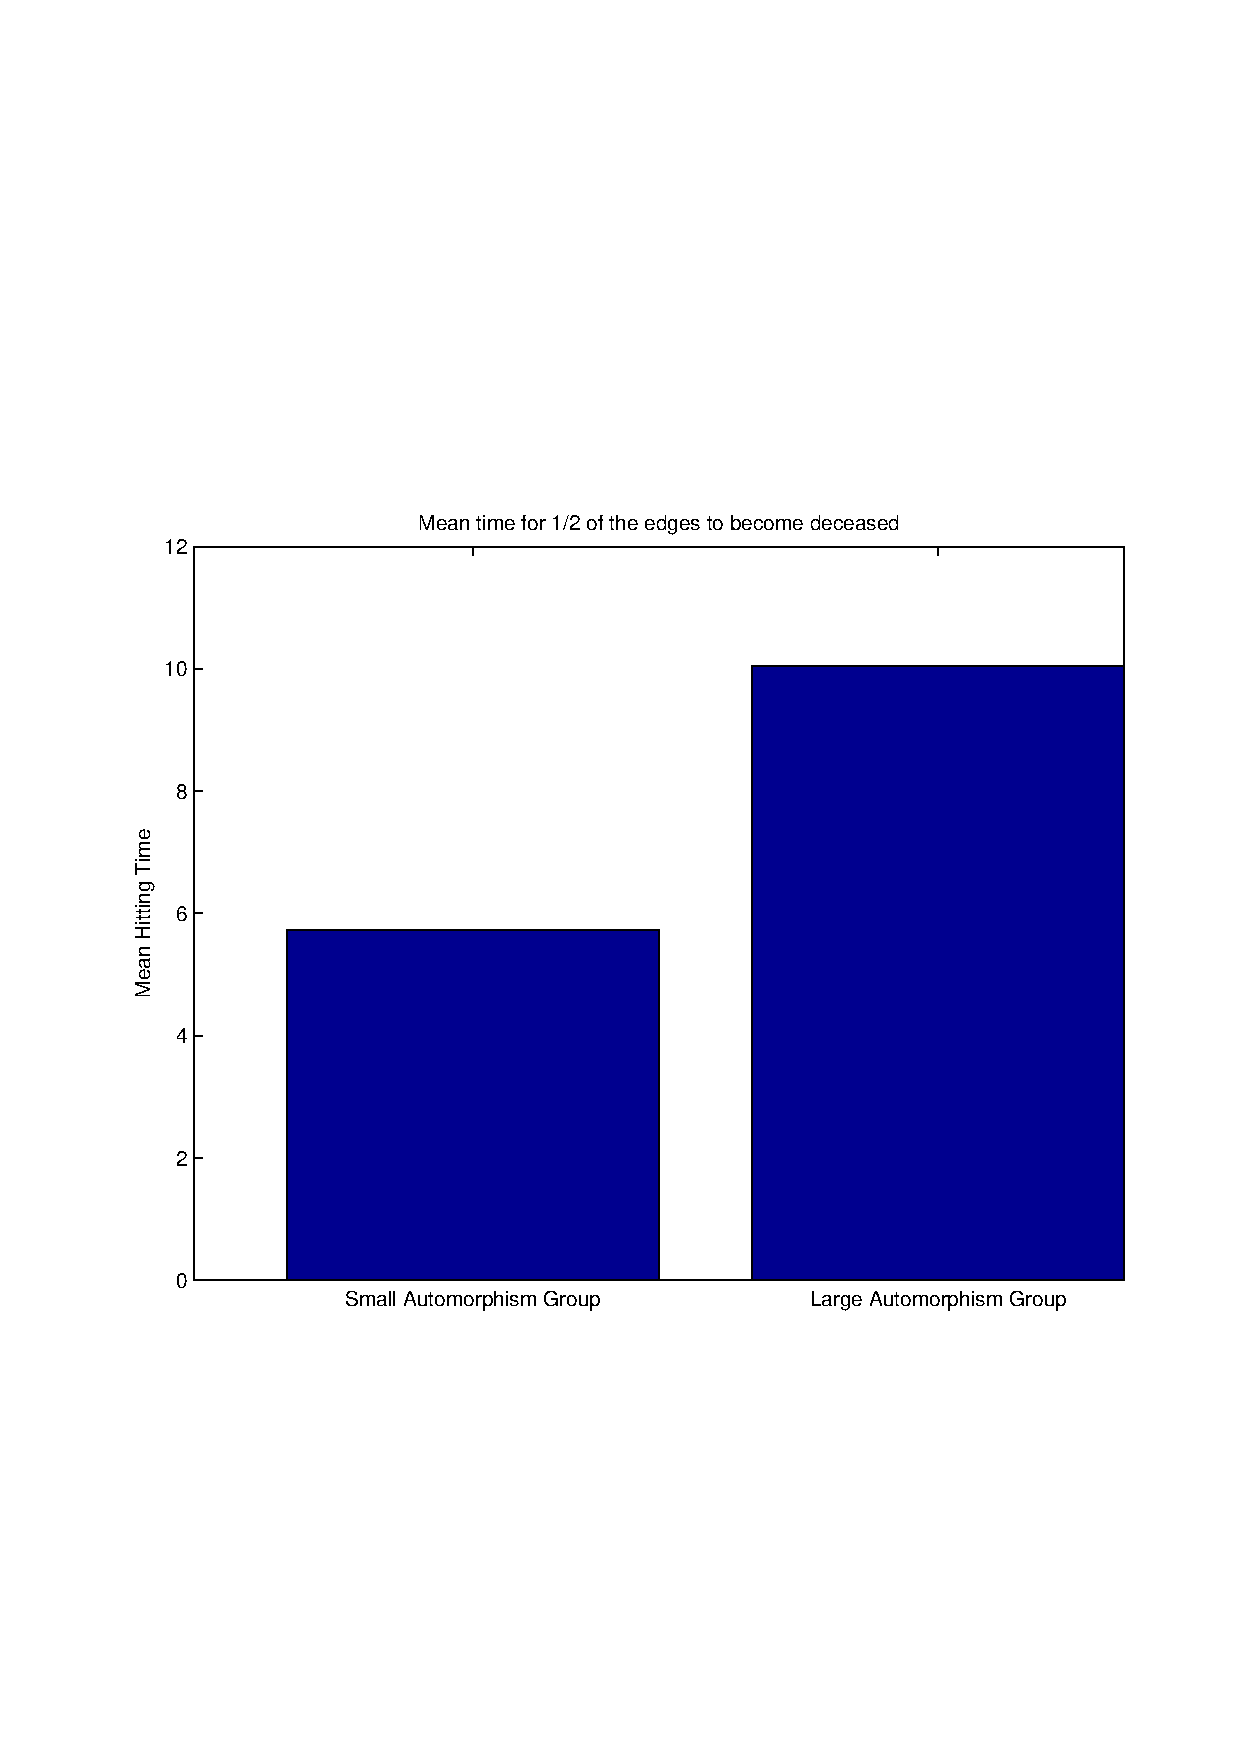
\includegraphics[scale=0.15]{halof.pdf}
                \caption{$\tau_{\frac{1}{2}}$.}\label{t12}
\end{figure}

For further corroboration we also defined $\tau_{\frac{2}{3}}$ and the corresponding $\mu_{1}'$ and $\mu_{2}'$.  

\begin{figure}[H]

              \centering
               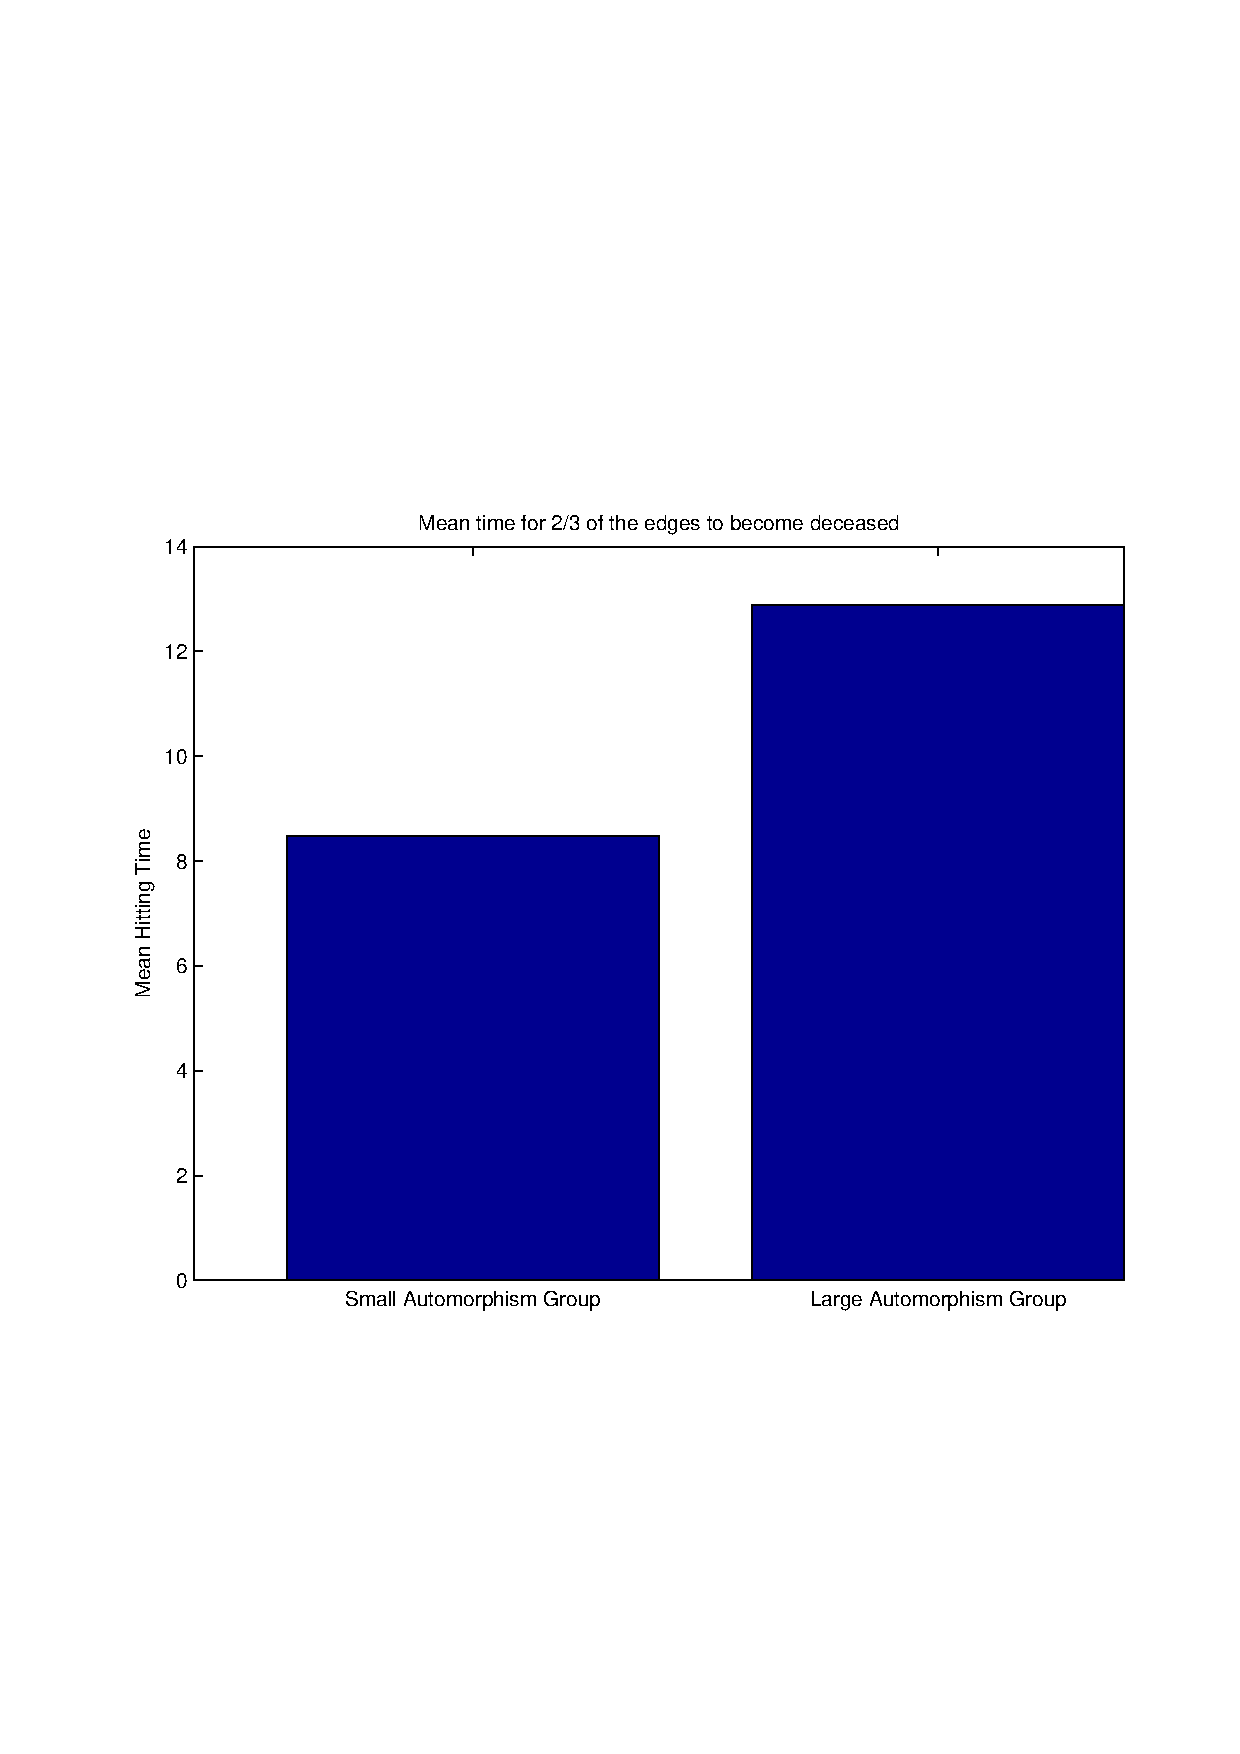
\includegraphics[scale=0.15]{twot.pdf}
                \caption{$\tau_{\frac{2}{3}}$.}\label{t23}
\end{figure}

The results show that the trees that were generated with a larger automorphism group had larger half and two thirds lives than the trees generated with smaller automorphism group.  

\subsection{Interpretation of results}

To understand the medical relevance of these results note that large $\tau_{\frac{1}{2}}$ means that it took longer for half of the vessels to be removed so the degree of CAA was less severe.  Our results suggest that a cerebral vascular structure that is highly symmetric (has a large automorphism group) is more \emph{robust} to CAA.  

High levels of symmetry have been shown to be advantageous in other networks.  For example Song \emph{et al.} create a mathematical model to study the evolution of a biochemical annotation network. They show that a fractal network (a graph with a high level of symmetry) is more robust  i.e. the removal of many nodes has minimal effect on the shortest paths \cite{Song}.  

To gain some intuition as to why this is the case consider the following extreme example.  Let $T_{1}$ be the complete tree on 15 vertices and let $T_{2}$ be a line of 15 vertices as seen in Figure \ref{fig:silly}.  Notice that $|Aut(T_{1})| = BIG$ and that $|Aut(T_{2}|$ = 2 so $T_{1}$ is much more symmetric than $T_{2}$.  

\begin{figure}[H]
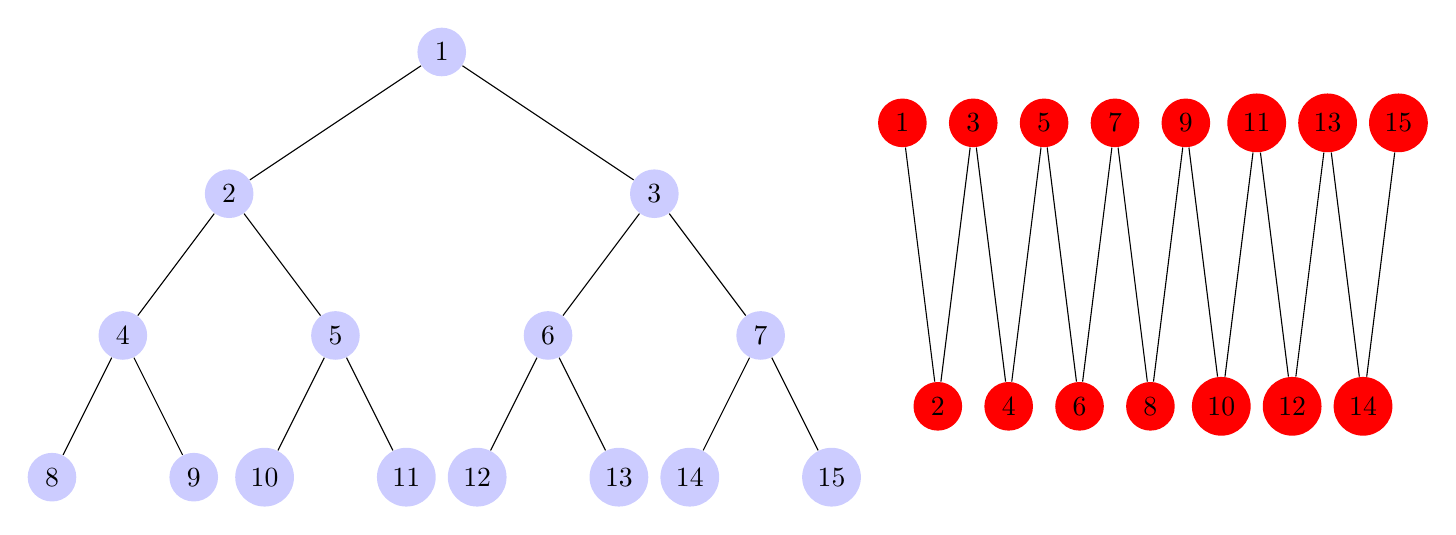
\begin{tikzpicture}
  [scale=0.9,auto=left,every node/.style={circle,fill=blue!20}]
  \node (n1) at (5.5,7) {1};
  \node (n2) at (2.5,5)  {2};
  \node (n3) at (8.5,5)  {3};
  \node (n4) at (1,3) {4};
  \node (n5) at (4,3)  {5};
  \node (n6) at (7,3)  {6};
\node (n7) at (10,3)  {7};
\node (n8) at (0,1)  {8};
\node (n9) at (2,1)  {9};
\node (n10) at (3,1)  {10};
\node (n11) at (5,1)  {11};
\node (n12) at (6,1)  {12};
\node (n13) at (8,1)  {13};
\node (n14) at (9,1)  {14};
\node (n15) at (11,1)  {15};

\node[style={circle,fill=red!100}] (n16) at (12,6)  {1};
\node[style={circle,fill=red!100}] (n17) at (12.5,2)  {2};
\node[style={circle,fill=red!100}] (n18) at (13,6)  {3};
\node[style={circle,fill=red!100}] (n19) at (13.5,2)  {4};
\node[style={circle,fill=red!100}] (n20) at (14,6)  {5};
\node[style={circle,fill=red!100}] (n21) at (14.5,2)  {6};
\node[style={circle,fill=red!100}] (n22) at (15,6)  {7};
\node[style={circle,fill=red!100}] (n23) at (15.5,2)  {8};
\node[style={circle,fill=red!100}] (n24) at (16,6)  {9};
\node[style={circle,fill=red!100}] (n25) at (16.5,2)  {10};
\node[style={circle,fill=red!100}] (n26) at (17,6)  {11};
\node[style={circle,fill=red!100}] (n27) at (17.5,2)  {12};
\node[style={circle,fill=red!100}] (n28) at (18,6)  {13};
\node[style={circle,fill=red!100}] (n29) at (18.5,2)  {14};
\node[style={circle,fill=red!100}] (n30) at (19,6)  {15};

  \foreach \from/\to in {n1/n2,n1/n3,n2/n4,n2/n5,n3/n6,n3/n7,n4/n8,n4/n9,n5/n10,n5/n11,n6/n12,n6/n13,n7/n14,n7/n15,n16/n17,n17/n18,n18/n19,n19/n20,n20/n21,n21/n22,n22/n23,n23/n24,n24/n25,n25/n26,n26/n27,n27/n28,n28/n29,n29/n30}
    \draw (\from) -- (\to);

\end{tikzpicture}
\caption{$T_{1}$ and $T_{2}$}\label{fig:silly}
\end{figure}
If we remove an edge at random from $T_{1}$ and also remove the  induced subtree adjacent to that edge the expected number of edges removed is:
\begin{equation}
1\frac{8}{14} + 3\frac{4}{14} + 7\frac{2}{14} = \frac{12}{7} 
\end{equation} 
If we remove an edge at random from $T_{2}$ and also remove the  induced subtree adjacent to that edge the expected number of edges removed is:
\begin{equation}
\frac{1}{14}\sum_{k=1}^{14}k = \frac{15}{2} > \frac{12}{7}
\end{equation}

One could argue that our results were the result of weak assumptions regarding concentration, however we yielded a similar result with a simplified experiment.  We built 50 random recursive binary trees $\mathcal{T}$ in the same way and set $P$ to be constant rather than a function of concentration.  We split $\mathcal{T}$ into $\mathcal{T}_{1}$ and $\mathcal{T}_{2}$ and found the mean hitting times $\mu_{1}$ and $\mu_{2}$.  Again we found that $\mu_{1} < \mu_{2}$.  

\section{Conclusions and Further Directions}
In order to improve the accuracy of our model we could make several modifications.  Firstly, Ambrose has shown that the brain undergoes angiogenisis  (the creation of new arterial vessels) which could be reflected in the model by adding edges at random.  Further we could modify the deletion process by going from a model in which an edge either exists or does not to a model in which each edge allows a variable flow which decreases at random.  We could also attempt to reflect the fact that modelling the basement membranes as annular prisms does not take into account the tortuous routes of perivascular drainage.  Finally, we could also model the stiffening of arteries over time  by introducing a radial function that monotonically decreases.

We have demonstrated that it is likely that there is correlation between symmetry of the cerebral vascularture and lower risk of proliferation of CAA.  Further evidence of this correlation could be found by examining the relationship between highly symmetric areas of the brain and the extent to which those areas are affected by CAA.  

\bibliographystyle{h-physrev3.bst}
%\bibliographystyle{plain}

\bibliography{./medicine}

\end{document}
